\chapter{Experiments and Result}
\section{Multiplier Block: Squaring Block Test Schematics}
At first we've tested the performance of the Squaring Block.

\begin{figure}[h]
	\centering
	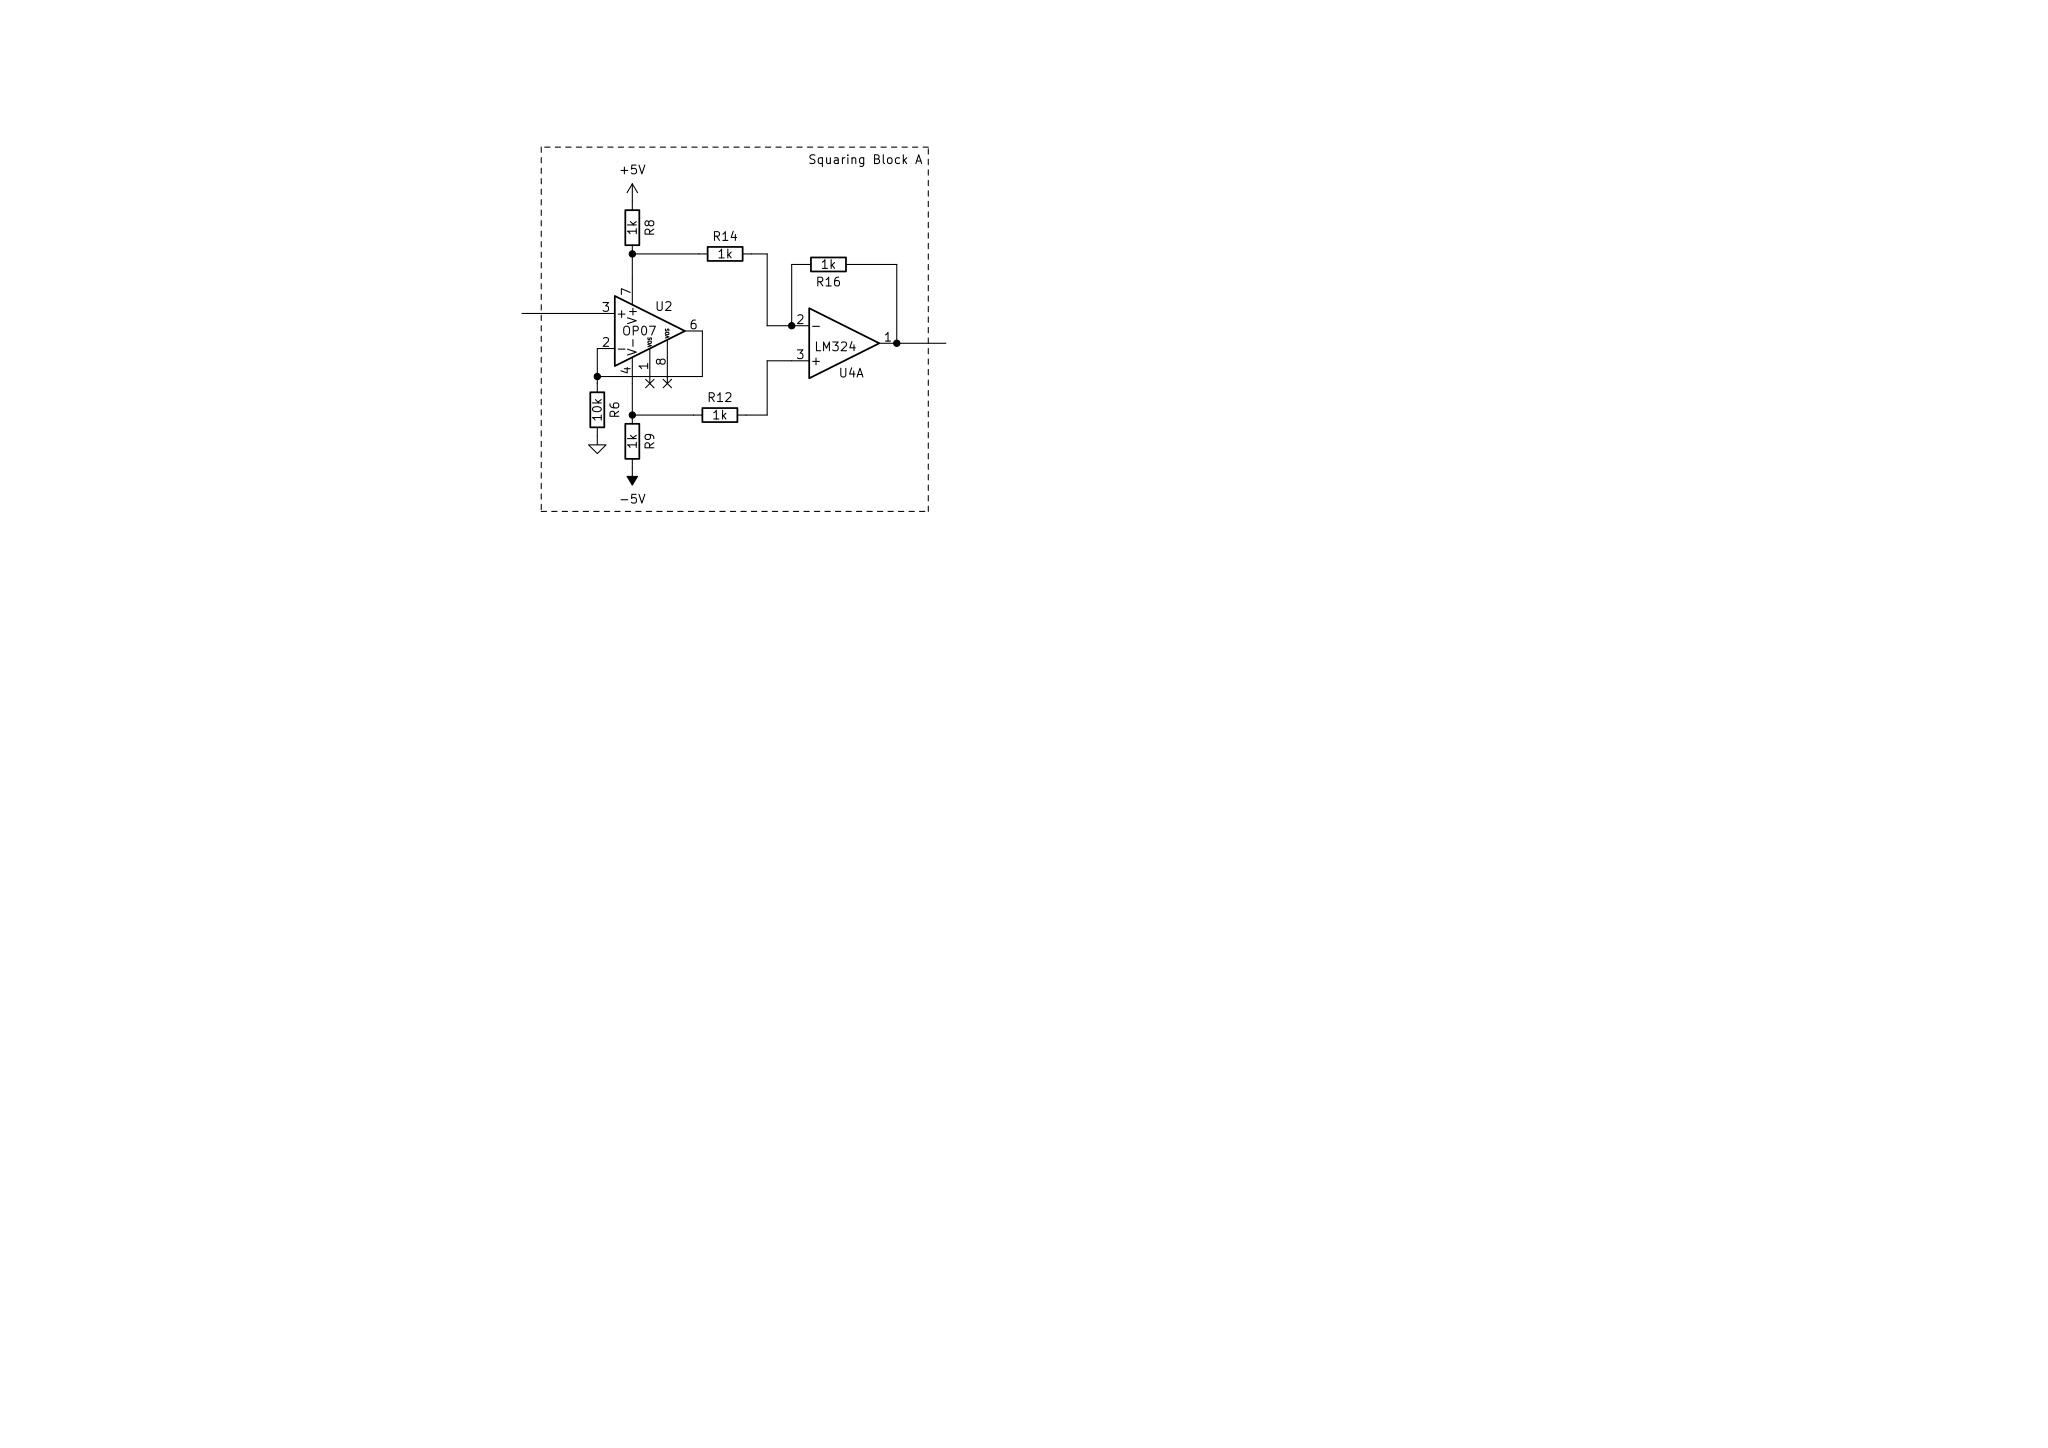
\includegraphics[width=3in]{fig/ckt6.eps}
	\caption{Multiplier Block}
	\label{ckt5}
\end{figure}

We have measured the DC Transfer characteristics. The results are listed below.

\vspace{1cm}
\begin{tabular}{c c c}
	Observation & Input Voltage ($ V_{in} $) (mV) & Output Voltage ($ V_{out} $) (mV)\\
	\hline
	1	&	508 &	237\\
	2	&	598	&	276\\
	3	&	682	&	313\\
	4	&	760	&	349\\
	5	& 	837	&	379\\
	6	&	915	&	413\\
	7	&	985	&	449
\end{tabular}
\begin{figure}[h]
	\centering
	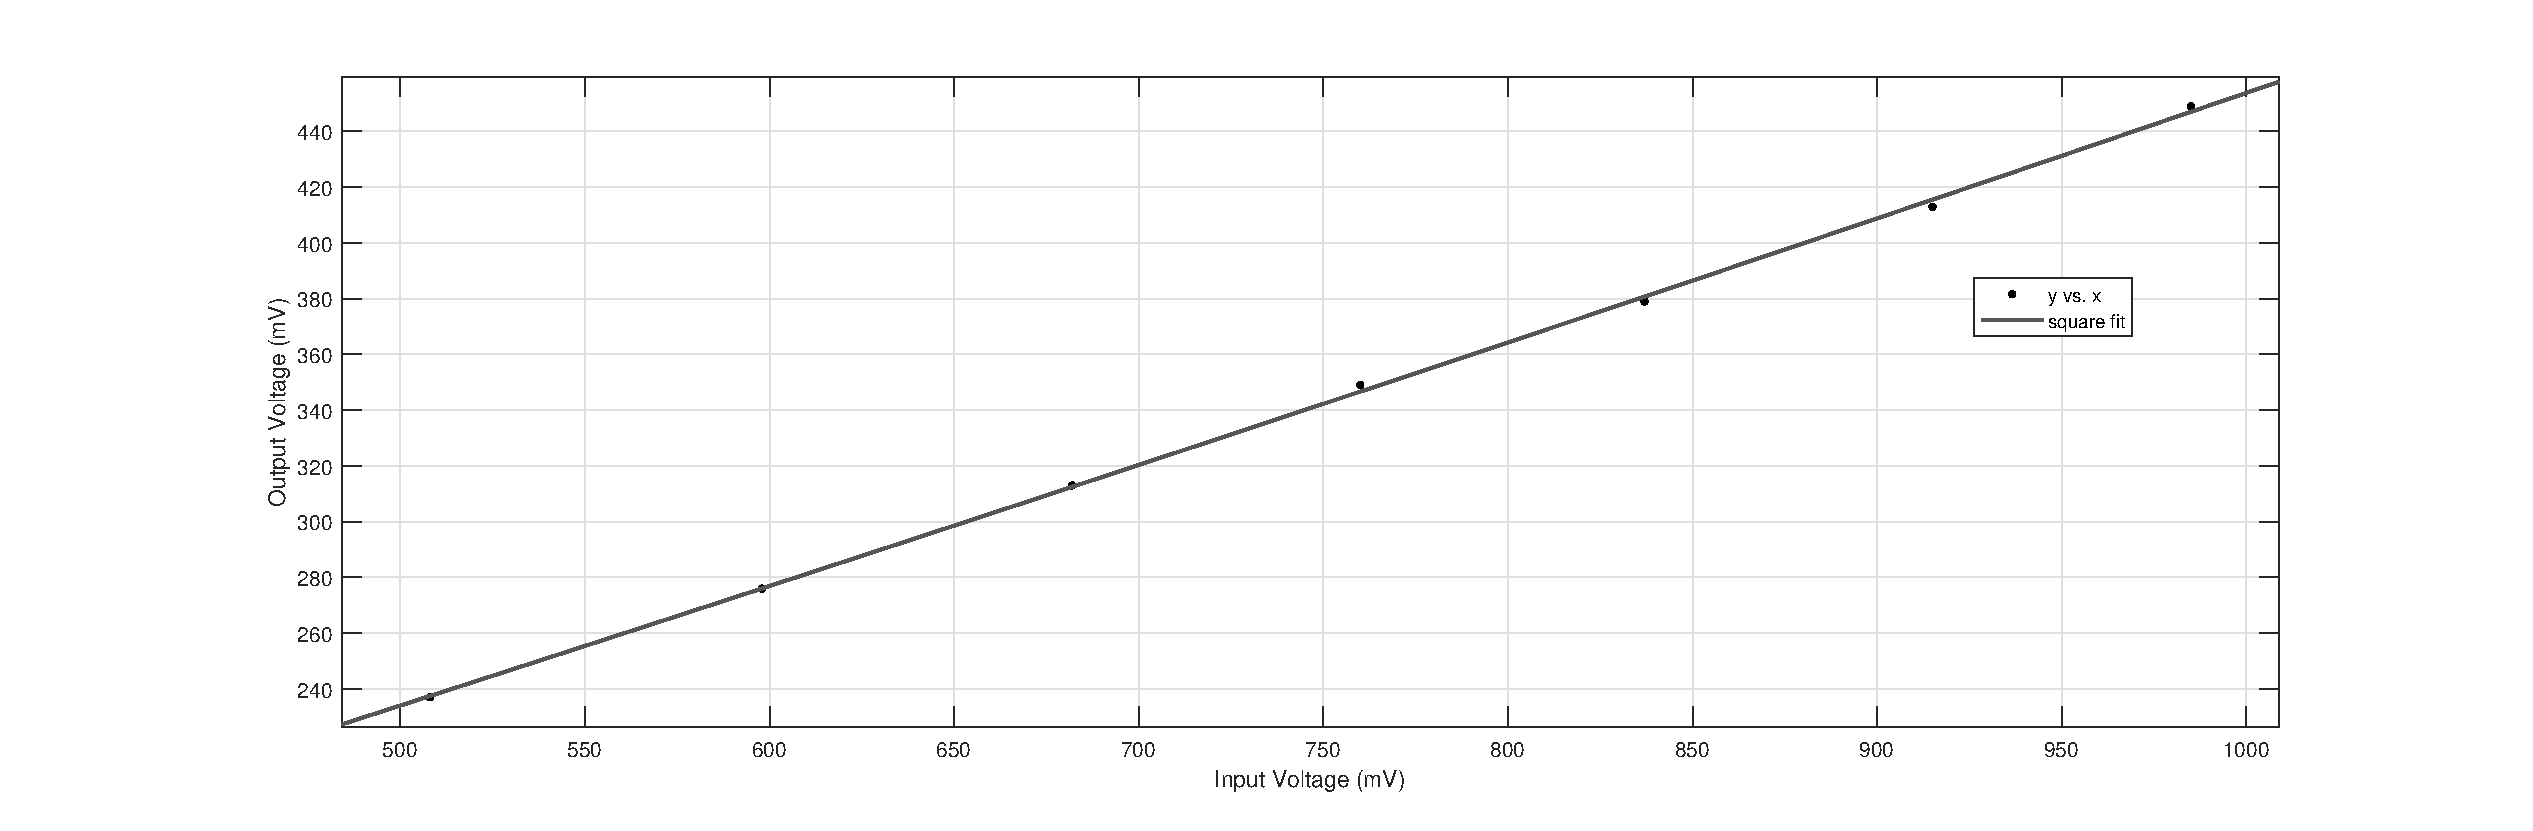
\includegraphics[width=\columnwidth]{fig/plt1.eps}
	\caption{DC Transfer Characteristics.}
	\label{plt1}
\end{figure}

\section{Multiplier Block: Full Test Schematics}
This is the exact circuit which we used to test our prototype.
\begin{figure}[h]
	\centering
	\includegraphics[width=\columnwidth]{fig/ckt5.eps}
	\caption{Multiplier Block}
	\label{ckt5}
\end{figure}

\newpage
\section{Matrix Multiplication (Partial): Full Test Schematics}
For a prototype, we chose a $ 2 \times 2 $ matrix multiplication and computed only the element of the first-row-first-column.

\begin{figure}[h]
	\centering
	\includegraphics[width=\columnwidth]{fig/ckt7.eps}
	\caption{Generating output of the first cell of resulting matrix.}
	\label{ckt7}
\end{figure}